\documentclass[a5paper, 12pt]{scrartcl}

\usepackage[europeanresistors]{circuitikz}
\usepackage{siunitx}
\usepackage{lipsum, mystyle}

\usepackage{scrlayer-scrpage}

\clearpairofpagestyles{}

\setkomafont{pageheadfoot}{\sffamily\footnotesize}
\setkomafont{pagination}{}

\ohead{Seite~\pagemark}
\ihead{Emil Slomka, Tim Hilt}

\KOMAoptions{
  headsepline=true,
}

\begin{document}

\newgeometry{left=1cm, right=1cm, top=2cm, bottom=1cm}
\begin{center}
  \usekomafont{disposition}\huge Elektronik Formelsammlung
\end{center}

\section{Grundlagen und Wiederholung}

\begin{minipage}{.45\textwidth}
\textbf{Übertragungsfunktion:} \[F = \frac{U_a}{U_e} = \frac{\text{Widerstände parallel zum Ausgang}}{\text{Widerstände parallel zum Eingang}}\]

\textbf{Berechnung zweier, paralleler Widerstände \(R_1\) und \(R_2\):} \[R_1 || R_2 = \frac{R_1 \cdot R_2}{R_1 + R_2}\]

\textbf{Leistung:} \[P = \frac{U^2}{R} = U \cdot \frac{U}{R} = U \cdot I\]
\end{minipage}\hfill\vline\hfill%
\begin{minipage}{.45\textwidth}
  \lipsum[4]
\end{minipage}

\section{Kondensator und Zeitkonstanten}

Zeitkonstante \(\tau\) beim \mybfcol{Kondensator}: \dotfill \(\tau = R \cdot C\)\\
Zeitkonstante \(\tau\) bei der \mybfcol{Spule}: \dotfill \(\tau = \frac{L}{R}\)\\

\begin{figure}[H]
  \centering
  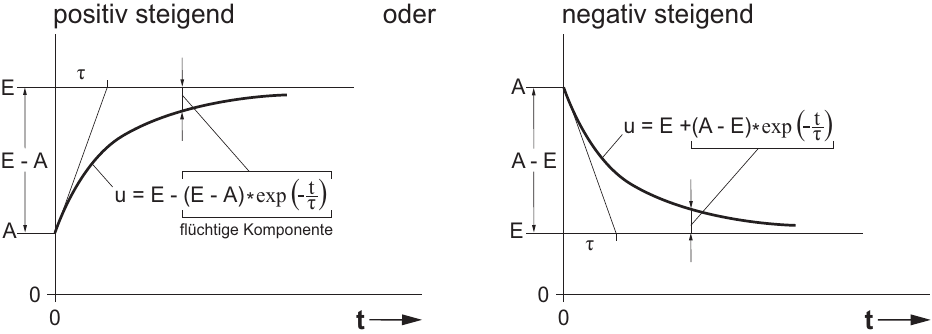
\includegraphics[width=.7\textwidth]{LadekurveKondensator}
  \caption{Ladekurven Kondensator \mybfcol{Achtung: \(t = \Delta t = t_1 - t_0\)}}
\end{figure}

\textbf{Zum Zeichnen im Zeitbereich:} Arbeitsgerade von Anfangsspannung zur Endspannung zeichnen, mit \(t = \tau\)

\mybfcol{Achtung: Immer alle Widerstände parallel und in Reihe zum Kondensator berücksichtigen und Übertragungsfunktion für Ladeziel verwenden!}

\begin{table}
  \centering
  \begin{tabular}{cc}
    \toprule
    \(t=\tau\) & \(\approx 63\%\) von\ \(|A-E|\)\\
    \(t=2\tau\) & \(\approx 86\%\) von\ \(|A-E|\)\\
    \(t=5\tau\) & \(\approx 99\%\) von\ \(|A-E|\)\\
    \bottomrule
  \end{tabular}
\end{table}

\section{Filter}

Im Fourierbereich: \(\omega = 2 \pi f\), im Laplacebereich: \(j\omega = p\)

\begin{table}[H]
  \centering
  \begin{tabular}{cllll}
    \toprule
    & \textbf{RC-Tiefpass} & \textbf{RC-Hochpass} & \textbf{RL-Tiefpass} & \textbf{RL-Hochpass}\\
    \midrule
    \textbf{Übertragungsfunktion \(\frac{U_a}{U_e} = H(j\omega)\)} & \(\frac{1}{1 + j\omega R C}\) & \(\frac{j\omega RC}{1 + j\omega RC}\) & \(\frac{R}{R + j \omega L}\)& \(\frac{j\omega L}{R + j \omega L}\) \\[1em]
    \textbf{Grenzfrequenz \(f_G / \omega_G\)} & \(\frac{1}{2 \pi R C}; \frac{1}{RC}\) & \(\frac{1}{2 \pi R C}; \frac{1}{RC}\) & \(\frac{R}{2 \pi L}; \frac{R}{L}\) & \(\frac{R}{2 \pi L}; \frac{R}{L}\)\\
    \bottomrule
  \end{tabular}
  \caption{Grenzfrequenz und Übertragungsfunktionen}
\end{table}

\textbf{Dämpfung bei passiven Filtern erster Ordnung:}

\begin{itemize}
\item \SI{0}{\decibel} im Durchlassbereich
\item \SI{3}{\decibel} an der Grenzfrequenz \(f_G\)
\item \SI{6}{\decibel} pro Oktave (doppelte Frequenz) im Sperrbereich
\item \SI{20}{\decibel} pro Dekade (zehnfache Frequenz) im Sperrbereich
\end{itemize}

\section{Transistor}

\begin{figure}[H]
  \centering
  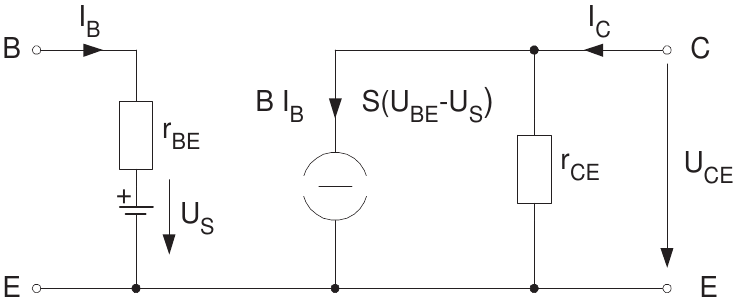
\includegraphics[width=.6\textwidth]{ESBTransistor}
  \caption{Gleichstromersatzschaltbild eines Bipolartransistors}
\end{figure}

\end{document}


%%% Local Variables:
%%% mode: latex
%%% TeX-master: t
%%% End:
